\chapter{Writing a Lojban parser}

\section{Introduction}

This chapter will explore the main reference for Lojban (\cite{cowan1997complete}), in its 2016 revised version, and write a parser for a subset of the language.

Format: Extended Backus-Naur form

Parser: PEG

https://pypi.org/project/parsimonious/

https://github.com/erikrose/parsimonious

\section{Preparatory work}

\subsection{Testing if the parser works}
\label{sub:testing_if_the_parser_works}

(See Appendix \ref{appendix:testing_the_parser} for the corresponding code annex)

\begin{figure}[H]
\hspace{-2cm}
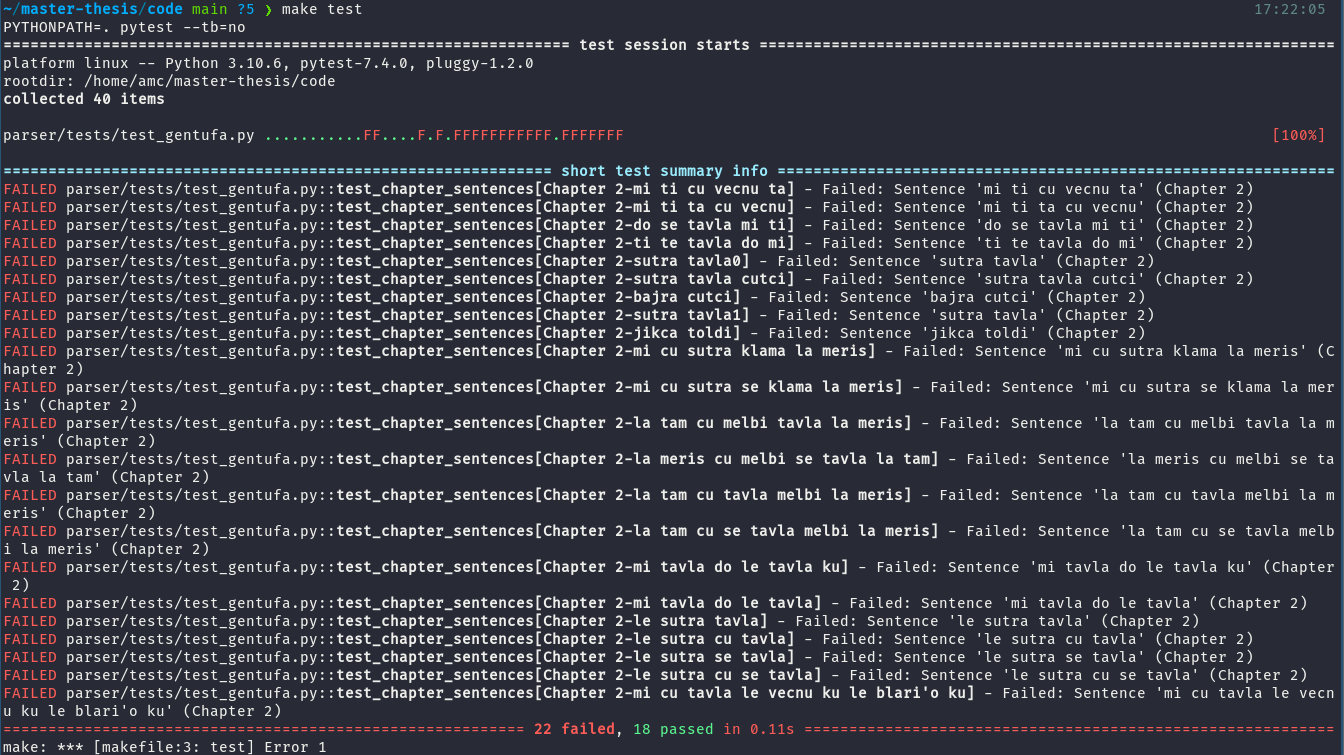
\includegraphics[scale=0.43]{images/pytest_output.png}
\caption{Pytest Output Example}
\end{figure}
